% Options for packages loaded elsewhere
\PassOptionsToPackage{unicode}{hyperref}
\PassOptionsToPackage{hyphens}{url}
%
\documentclass[
]{book}
\usepackage{amsmath,amssymb}
\usepackage{lmodern}
\usepackage{ifxetex,ifluatex}
\ifnum 0\ifxetex 1\fi\ifluatex 1\fi=0 % if pdftex
  \usepackage[T1]{fontenc}
  \usepackage[utf8]{inputenc}
  \usepackage{textcomp} % provide euro and other symbols
\else % if luatex or xetex
  \usepackage{unicode-math}
  \defaultfontfeatures{Scale=MatchLowercase}
  \defaultfontfeatures[\rmfamily]{Ligatures=TeX,Scale=1}
\fi
% Use upquote if available, for straight quotes in verbatim environments
\IfFileExists{upquote.sty}{\usepackage{upquote}}{}
\IfFileExists{microtype.sty}{% use microtype if available
  \usepackage[]{microtype}
  \UseMicrotypeSet[protrusion]{basicmath} % disable protrusion for tt fonts
}{}
\makeatletter
\@ifundefined{KOMAClassName}{% if non-KOMA class
  \IfFileExists{parskip.sty}{%
    \usepackage{parskip}
  }{% else
    \setlength{\parindent}{0pt}
    \setlength{\parskip}{6pt plus 2pt minus 1pt}}
}{% if KOMA class
  \KOMAoptions{parskip=half}}
\makeatother
\usepackage{xcolor}
\IfFileExists{xurl.sty}{\usepackage{xurl}}{} % add URL line breaks if available
\IfFileExists{bookmark.sty}{\usepackage{bookmark}}{\usepackage{hyperref}}
\hypersetup{
  pdftitle={IRTG COURSE: INTRODUCTION TO R},
  pdfauthor={Carl Herrmann \& Carlos Ramirez},
  hidelinks,
  pdfcreator={LaTeX via pandoc}}
\urlstyle{same} % disable monospaced font for URLs
\usepackage{color}
\usepackage{fancyvrb}
\newcommand{\VerbBar}{|}
\newcommand{\VERB}{\Verb[commandchars=\\\{\}]}
\DefineVerbatimEnvironment{Highlighting}{Verbatim}{commandchars=\\\{\}}
% Add ',fontsize=\small' for more characters per line
\usepackage{framed}
\definecolor{shadecolor}{RGB}{248,248,248}
\newenvironment{Shaded}{\begin{snugshade}}{\end{snugshade}}
\newcommand{\AlertTok}[1]{\textcolor[rgb]{0.94,0.16,0.16}{#1}}
\newcommand{\AnnotationTok}[1]{\textcolor[rgb]{0.56,0.35,0.01}{\textbf{\textit{#1}}}}
\newcommand{\AttributeTok}[1]{\textcolor[rgb]{0.77,0.63,0.00}{#1}}
\newcommand{\BaseNTok}[1]{\textcolor[rgb]{0.00,0.00,0.81}{#1}}
\newcommand{\BuiltInTok}[1]{#1}
\newcommand{\CharTok}[1]{\textcolor[rgb]{0.31,0.60,0.02}{#1}}
\newcommand{\CommentTok}[1]{\textcolor[rgb]{0.56,0.35,0.01}{\textit{#1}}}
\newcommand{\CommentVarTok}[1]{\textcolor[rgb]{0.56,0.35,0.01}{\textbf{\textit{#1}}}}
\newcommand{\ConstantTok}[1]{\textcolor[rgb]{0.00,0.00,0.00}{#1}}
\newcommand{\ControlFlowTok}[1]{\textcolor[rgb]{0.13,0.29,0.53}{\textbf{#1}}}
\newcommand{\DataTypeTok}[1]{\textcolor[rgb]{0.13,0.29,0.53}{#1}}
\newcommand{\DecValTok}[1]{\textcolor[rgb]{0.00,0.00,0.81}{#1}}
\newcommand{\DocumentationTok}[1]{\textcolor[rgb]{0.56,0.35,0.01}{\textbf{\textit{#1}}}}
\newcommand{\ErrorTok}[1]{\textcolor[rgb]{0.64,0.00,0.00}{\textbf{#1}}}
\newcommand{\ExtensionTok}[1]{#1}
\newcommand{\FloatTok}[1]{\textcolor[rgb]{0.00,0.00,0.81}{#1}}
\newcommand{\FunctionTok}[1]{\textcolor[rgb]{0.00,0.00,0.00}{#1}}
\newcommand{\ImportTok}[1]{#1}
\newcommand{\InformationTok}[1]{\textcolor[rgb]{0.56,0.35,0.01}{\textbf{\textit{#1}}}}
\newcommand{\KeywordTok}[1]{\textcolor[rgb]{0.13,0.29,0.53}{\textbf{#1}}}
\newcommand{\NormalTok}[1]{#1}
\newcommand{\OperatorTok}[1]{\textcolor[rgb]{0.81,0.36,0.00}{\textbf{#1}}}
\newcommand{\OtherTok}[1]{\textcolor[rgb]{0.56,0.35,0.01}{#1}}
\newcommand{\PreprocessorTok}[1]{\textcolor[rgb]{0.56,0.35,0.01}{\textit{#1}}}
\newcommand{\RegionMarkerTok}[1]{#1}
\newcommand{\SpecialCharTok}[1]{\textcolor[rgb]{0.00,0.00,0.00}{#1}}
\newcommand{\SpecialStringTok}[1]{\textcolor[rgb]{0.31,0.60,0.02}{#1}}
\newcommand{\StringTok}[1]{\textcolor[rgb]{0.31,0.60,0.02}{#1}}
\newcommand{\VariableTok}[1]{\textcolor[rgb]{0.00,0.00,0.00}{#1}}
\newcommand{\VerbatimStringTok}[1]{\textcolor[rgb]{0.31,0.60,0.02}{#1}}
\newcommand{\WarningTok}[1]{\textcolor[rgb]{0.56,0.35,0.01}{\textbf{\textit{#1}}}}
\usepackage{longtable,booktabs,array}
\usepackage{calc} % for calculating minipage widths
% Correct order of tables after \paragraph or \subparagraph
\usepackage{etoolbox}
\makeatletter
\patchcmd\longtable{\par}{\if@noskipsec\mbox{}\fi\par}{}{}
\makeatother
% Allow footnotes in longtable head/foot
\IfFileExists{footnotehyper.sty}{\usepackage{footnotehyper}}{\usepackage{footnote}}
\makesavenoteenv{longtable}
\usepackage{graphicx}
\makeatletter
\def\maxwidth{\ifdim\Gin@nat@width>\linewidth\linewidth\else\Gin@nat@width\fi}
\def\maxheight{\ifdim\Gin@nat@height>\textheight\textheight\else\Gin@nat@height\fi}
\makeatother
% Scale images if necessary, so that they will not overflow the page
% margins by default, and it is still possible to overwrite the defaults
% using explicit options in \includegraphics[width, height, ...]{}
\setkeys{Gin}{width=\maxwidth,height=\maxheight,keepaspectratio}
% Set default figure placement to htbp
\makeatletter
\def\fps@figure{htbp}
\makeatother
\setlength{\emergencystretch}{3em} % prevent overfull lines
\providecommand{\tightlist}{%
  \setlength{\itemsep}{0pt}\setlength{\parskip}{0pt}}
\setcounter{secnumdepth}{5}
\ifluatex
  \usepackage{selnolig}  % disable illegal ligatures
\fi
\usepackage[]{biblatex}

\title{IRTG COURSE: INTRODUCTION TO R}
\author{Carl Herrmann \& Carlos Ramirez}
\date{14 June, 2021}

\begin{document}
\maketitle

{
\setcounter{tocdepth}{1}
\tableofcontents
}
\hypertarget{intro}{%
\chapter{scRNA-Seq Course Syllabus}\label{intro}}

We will use available data from 10X genomics of Peripheral Blood Mononuclear cells (PBMC). In order
to speed up the process only a subset of 500 cells are going to be processed here. Here, we will
perform the following tasks:

\begin{itemize}
\tightlist
\item
  Definition of a Seurat object from a matrix of counts
\item
  Quality Control (QC) of the cell samples
\item
  Filtering
\item
  Dimensional reduction
\item
  Clustering
\item
  Differential expression
\item
  Visualization of markers
\end{itemize}

\hypertarget{single-cell-sequencing}{%
\section{Single Cell Sequencing}\label{single-cell-sequencing}}

Single cell sequencing (scRNA-Seq) technologies arise from bulk counterparts with
the aim of refining gene expression profiles. Previous bulk Sequencing offered
averaged quantifications of gene expression in samples. In some contexts, for
example, when studying cell type specificity or the heterogeneity in tumours is
important to dissect patterns in cell subpopulations.

The following image illustrates the development of scRNA-Seq technologies
and the number of cells that can be analyzed with each technology. In this
course we will not discuss platform sequencing technologies in detail,
instead we will take a hands on approach and jump directly to the analysis
of scRNA-Seq data. However, the analysis that we show next are applied downstream
to libraries construction or sequencing, and are therefore platform agnostic.

\begin{figure}
\centering
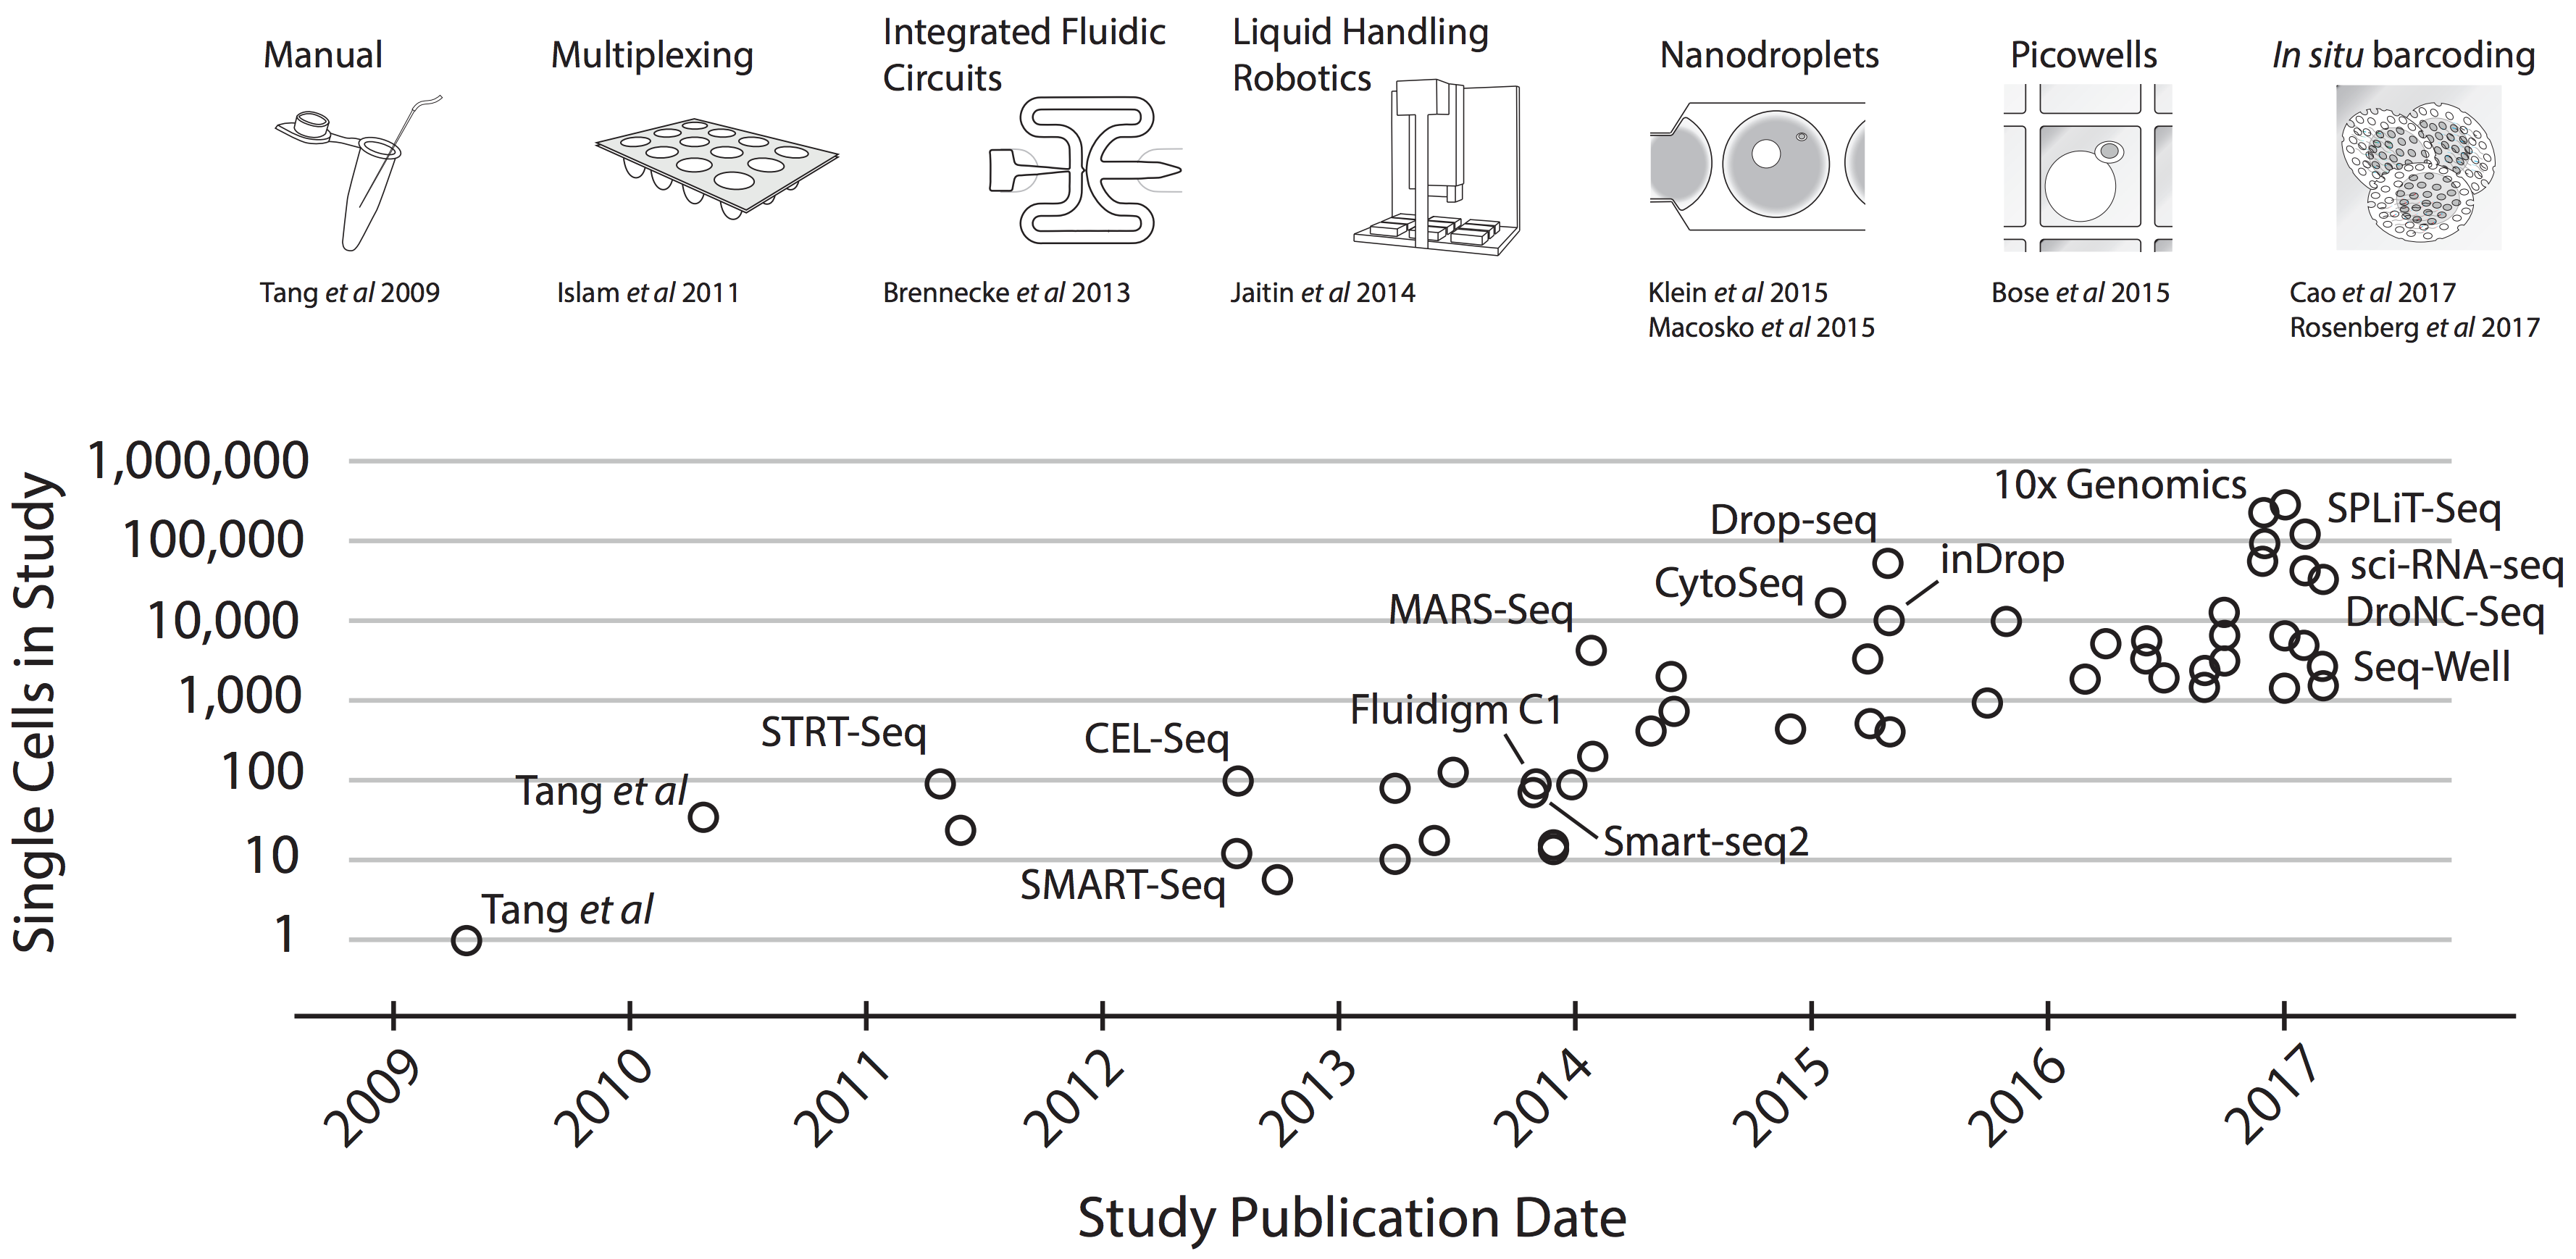
\includegraphics{figures/moores-law.png}
\caption{\textbf{Single Cell Sequencing Platforms}: Date of development \emph{vs} number of cells analyzed by each technology.}
\end{figure}

The image is taken from \href{https://arxiv.org/abs/1704.01379}{Svensson V et al, 2017}.

\hypertarget{quantifying-gene-expression-in-single-cells}{%
\section{Quantifying gene expression in single cells}\label{quantifying-gene-expression-in-single-cells}}

Genes are expressed in cells by the synthesis of mRNA molecules. Quantification of gene expression
in single cells consists of counting and mapping sequenced reads to each gene in each cell. The
outcome of this process is a count matrix, which is a discrete matrix of integers corresponding
to the number of RNA molecules associated to each gene and cell. The count matrix usually has
genes as rows and cells in columns.

In the next lines we will load the matrix of UMI counts into a variable called \texttt{pbmc.mtx}.

\begin{Shaded}
\begin{Highlighting}[]
\DocumentationTok{\#\# Loading example data}
\NormalTok{pbmc\_url  }\OtherTok{\textless{}{-}} \StringTok{\textquotesingle{}https://github.com/caramirezal/caramirezal.github.io/raw/master/bookdown{-}minimal/data/pbmc\_10X\_500\_cells.mtx.rds\textquotesingle{}}
\NormalTok{pbmc.mtx }\OtherTok{\textless{}{-}} \FunctionTok{readRDS}\NormalTok{(}\FunctionTok{url}\NormalTok{(pbmc\_url))}
\end{Highlighting}
\end{Shaded}

As can be seen from the output of the function \texttt{dim(pbmc.mtx)} the matrix contains 13,714 rows (genes) and columns (cells).

\begin{Shaded}
\begin{Highlighting}[]
\FunctionTok{dim}\NormalTok{(pbmc.mtx)}
\end{Highlighting}
\end{Shaded}

\begin{verbatim}
## [1] 13714   500
\end{verbatim}

To have a glimpse of the appearance of this matrix we print the first 5 rows and first 5 columns. It can
be seen that the matrix object is a particular array called sparse Matrix. These types of matrices are
specially efficient to store numerical arrays which are very sparse (full of zeroes) as is the case
for single cell count matrices data.

\begin{Shaded}
\begin{Highlighting}[]
\NormalTok{pbmc.mtx[}\DecValTok{1}\SpecialCharTok{:}\DecValTok{5}\NormalTok{, }\DecValTok{1}\SpecialCharTok{:}\DecValTok{5}\NormalTok{]}
\end{Highlighting}
\end{Shaded}

\begin{verbatim}
## 5 x 5 sparse Matrix of class "dgCMatrix"
##               AAAGAGACGGACTT-1 AAAGATCTGGGCAA-1 AAAGCAGATATCGG-1
## AL627309.1                   .                .                .
## AP006222.2                   .                .                .
## RP11-206L10.2                .                .                .
## RP11-206L10.9                .                .                .
## LINC00115                    .                .                .
##               AAAGTTTGATCACG-1 AAATCAACCCTATT-1
## AL627309.1                   .                .
## AP006222.2                   .                .
## RP11-206L10.2                .                .
## RP11-206L10.9                .                .
## LINC00115                    .                .
\end{verbatim}

We can start from different types of arrays apart from sparse matrices as data frames or hd5
objects, just to give some examples. The format in which the matrix is provided might also vary from
excel files, tsv, csv, rds, etc. Usually this formats can be converted into each other, however, the
methods for such transformation are so different and specific that we cannot covered here all of them
here.

\hypertarget{quizzes}{%
\section{Quizzes}\label{quizzes}}

\begin{quote}
Manipulation of count matrices
\end{quote}

\emph{What is the mean and median number of UMI counts in these cells?}
a) median = 301, mean = 343
b) median = 11304, mean = 10432
c) median = 2216, mean = 2354

Answer:
\texttt{umi.sum\ \textless{}-\ apply(pbmc.mtx,\ 2,\ sum)}
\texttt{summary(umi.sum)}

\texttt{Min.\ 1st\ Qu.\ \ Median\ \ \ \ Mean\ 3rd\ Qu.\ \ \ \ Max.}
\texttt{561\ \ \ \ \ \ 1741\ \ \ \ \ \ 2216\ \ \ \ \ \ 2354\ \ \ \ \ \ 2746\ \ \ \ \ \ 7928}

\emph{What are the top genes with highest number of UMI counts in decreasing order?}
a) MALAT1, B2M, TMSB4X, RPL10, RPL13, RPL13A
b) RPL13, MALAT1, B2M, TMSB4X, RPL10, RPL13A
c) B2M, TMSB4X, RPL13A, RPL10, RPL13, MALAT1

Answer:
\texttt{\#\#\ Getting\ sum\ of\ umi\ counts\ per\ row\ (gene)}
\texttt{umi.sum.gene\ \textless{}-\ apply(pbmc.mtx,\ 1,\ sum)}

\texttt{\#\#\ Sorting\ and\ showing\ top\ 6\ genes\ with\ highest\ number\ of\ UMIs}
\texttt{sort(umi.sum.gene,\ decreasing\ =\ TRUE)\ \%\textgreater{}\%\ head()}
\texttt{MALAT1\ \ \ \ B2M\ TMSB4X\ \ RPL10\ \ RPL13\ RPL13A}
\texttt{28672\ \ 22976\ \ 22741\ \ 16616\ \ 14179\ \ 13975}

\hypertarget{standard-preprocessing-using-seurat}{%
\chapter{Standard Preprocessing using Seurat}\label{standard-preprocessing-using-seurat}}

Placeholder

\hypertarget{creating-seurat-object}{%
\section{Creating Seurat object}\label{creating-seurat-object}}

\hypertarget{exploring-the-seurat-object}{%
\section{Exploring the Seurat object}\label{exploring-the-seurat-object}}

\hypertarget{extracting-expression-values}{%
\section{Extracting expression values}\label{extracting-expression-values}}

\hypertarget{quizzes-1}{%
\section{Quizzes}\label{quizzes-1}}

\hypertarget{exercises}{%
\section{Exercises}\label{exercises}}

\hypertarget{quality-control}{%
\chapter{Quality control}\label{quality-control}}

Placeholder

\hypertarget{filtering-out-cells}{%
\section{Filtering out cells}\label{filtering-out-cells}}

\hypertarget{quizzes-2}{%
\section{Quizzes}\label{quizzes-2}}

\hypertarget{exercises-1}{%
\section{Exercises}\label{exercises-1}}

\hypertarget{feature-selection}{%
\chapter{Feature selection}\label{feature-selection}}

Placeholder

\hypertarget{exercises-2}{%
\section{Exercises}\label{exercises-2}}

\hypertarget{dimensional-reduction}{%
\chapter{Dimensional Reduction}\label{dimensional-reduction}}

Placeholder

\hypertarget{normalization}{%
\section{Normalization}\label{normalization}}

\hypertarget{dimensional-reduction-1}{%
\section{Dimensional reduction}\label{dimensional-reduction-1}}

\hypertarget{exercises-3}{%
\section{Exercises}\label{exercises-3}}

\hypertarget{cell-clustering}{%
\chapter{Cell clustering}\label{cell-clustering}}

Placeholder

\hypertarget{exercises-4}{%
\section{Exercises}\label{exercises-4}}

\hypertarget{umap}{%
\section{UMAP}\label{umap}}

\hypertarget{exercise}{%
\section{Exercise}\label{exercise}}

\hypertarget{differential-expression-analysis}{%
\chapter{Differential Expression Analysis}\label{differential-expression-analysis}}

Placeholder

\hypertarget{exercises-5}{%
\section{Exercises}\label{exercises-5}}

\hypertarget{markers-visualization}{%
\chapter{Markers visualization}\label{markers-visualization}}

Placeholder

\hypertarget{visualization-of-gene-expression-levels-of-markers-in-clusters}{%
\section{Visualization of gene expression levels of markers in clusters}\label{visualization-of-gene-expression-levels-of-markers-in-clusters}}

\hypertarget{exercises-6}{%
\section{Exercises}\label{exercises-6}}

\printbibliography

\end{document}
